\ifx\boi\undefined\ifx\problemname\undefined
\providecommand\sampleinputname{}
\providecommand\sampleoutputname{}
\documentclass[icelandic]{templates/boi}
\problemlanguage{.is}
\fi
\newcommand{\boi}{Eystrasaltsólympíuleikarnir í forritnu}
\newcommand{\practicesession}{Æfingakeppni}
\newcommand{\contestdates}{27. apríl - 1. maí, 2018}
\newcommand{\dayone}{Dagur 1}
\newcommand{\daytwo}{Dagur 2}
\newcommand{\licensingtext}{This problem is licensed under CC BY-SA 4.0.}
\newcommand{\problem}{Verkefni}
\newcommand{\inputsection}{Inntak}
\newcommand{\outputsection}{Úttak}
\newcommand{\interactivity}{Gagnvirkni}
\newcommand{\grading}{Flokkun}
\newcommand{\scoring}{Stigagjöf}
\newcommand{\constraints}{Takmarkanir}
\renewcommand{\sampleinputname}{Sýnidæmis inntak}
\renewcommand{\sampleoutputname}{Sýnidæmis úttak}
\newcommand{\sampleexplanation}[1]{Útskýring á sýnidæmi #1}
\newcommand{\sampleexplanations}{Útskýringar á sýnidæmum}
\newcommand{\timelimit}{Tímamörk}
\newcommand{\memorylimit}{Minnismörk}
\newcommand{\seconds}{s}
\newcommand{\megabytes}{MB}
\newcommand{\group}{Hópur}
\newcommand{\points}{Stig}
\newcommand{\limitsname}{Takmarkanir}
\newcommand{\additionalconstraints}{Auka takmarkanir}
\newcommand{\testgroups}{
Lausnin þín verður prófuð á einhvern fjölda prufuhópa, hver hópur gefur einhvern fjölda stiga.
Hver hópur inniheldur einhvern fjölda prufutilvika.
Til að fá stig fyrir hóp þarftu að leysa öll prufutilvik innan hópsins.
Lokastigin eru fengin úr skilunum sem gáfu hæst stig.
}
\fi
\def\version{jury-1}
\problemname{Ástarmarghyrningur}
Eins og við vitum öll geta sápuóperur með mörgum persónum leitt að alvarlega flóknu ástar drama.
Í sérstakri þáttaröð eru $N$ persónur. Hver persóna elskar nákvæmlega eina persónu (sem getur verið hún sjálf).
Við segjum að tvær persónur eru í sambandi ef og aðeins ef þær elska hvora aðra.

Ein týpa af flækingum kallast ``ástarmarghyrningur''.
Við segjum að þrjár eða fleiri persónur eru í ``ástarmarghyrning'' ef að fyrsta persónan elskar aðra, önnu elskar þá
þriðju og svo framvegis, og einnig að síðasta persónan elski þá fyrstu.

Nýlegar kannannir hafa sýnt fram á að áhorfendur séu þreyttir á þessu drama og vilja eitthvað rómantískara.
Því var ákveðið að skjóta einhverjar persónur með ástarörvum þannig að allir byrji í sambandi.
Með því að skjóta einhvern með ástarör er hægt að breyta hvaða persónu hann elskar (í hvaða persónu sem þú vilt).

Hver er minnsti fjöldi ástarörva sem þarf til að koma öllum í samband?

\section*{\inputsection}
Fyrsta línan inniheldur heiltöluna $N$, fjöldi persónna í þáttaröðinni.
Næstu $N$ línur innihalda tvö nöfn aðskilin með bili, $s$ og $t$, sem þýðir að persónan sem heitir $s$ elskar persónuna sem heitir $t$.
Nöfn persónna eru í mesta lagi $10$ stafir á lengd og innihalda aðeins enska lágstafi.

\section*{\outputsection}
Skrifaðu út eina heiltölu -- minnsta fjölda ástarörva sem þarf til að koma öllum í samband. Ef það er ekki hægt skrifaðu út \texttt{-1}.

\section*{\constraints}
\testgroups

\noindent
\begin{tabular}{| l | l | l | l |}
\hline
\group & \points & \limitsname & \additionalconstraints \\ \hline
1     & 21     & $2 \le N \le 20$ & \\ \hline
2     & 25     & $2 \le N \le 100\,000$ & Hver persóna er elskuð af einhverjum (mögulega þeim sjálfum). \\ \hline
3     & 29     & $2 \le N \le 100\,000$ & Það eru engin sambönd né ``ástarmarghyrningar'' \\ \hline
4     & 25     & $2 \le N \le 100\,000$ & \\ \hline
\end{tabular}

\section*{\sampleexplanations}

\begin{center}
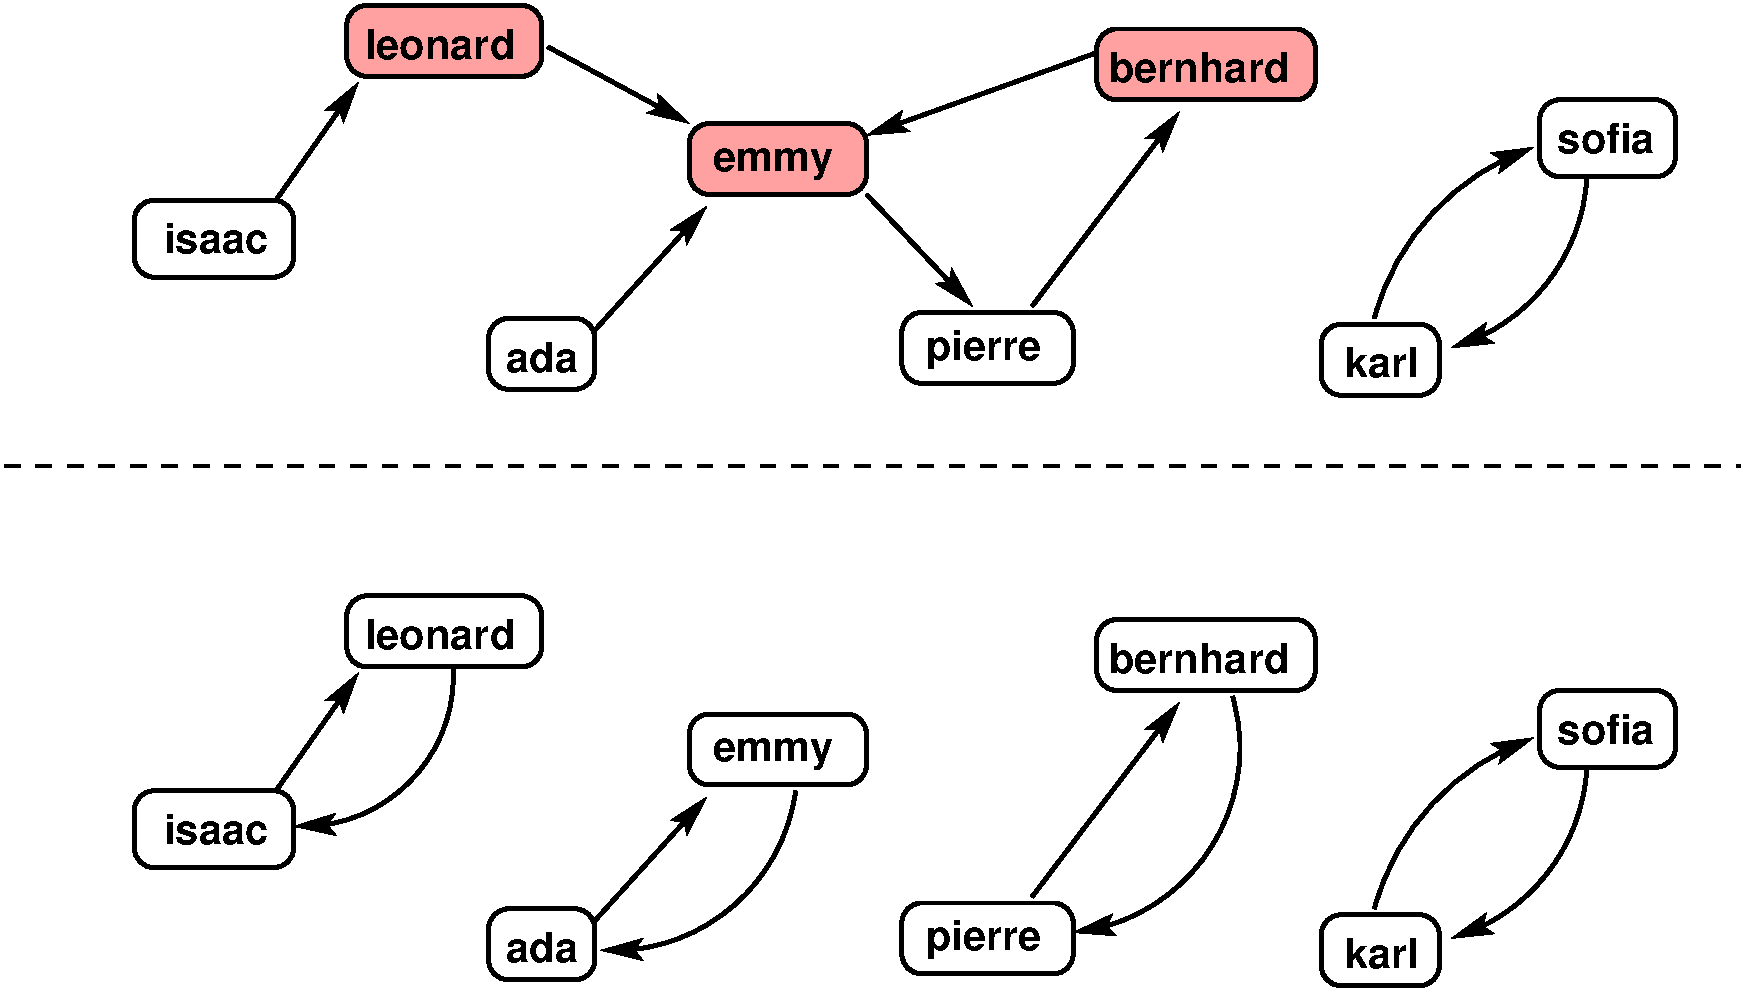
\includegraphics[width=0.5\textwidth]{polygonfig.pdf}
\end{center}

%In the first example, there is a unique optimal solution: shoot 
%which consists of shooting \texttt{b}, \texttt{d} and \texttt{f} with love arrows, having them fall in love with \texttt{h}, \texttt{c} and \texttt{e}, respectively.

Fyrsta sýnidæmið má sjá í myndinni að ofan. Efri parturinn sýnir upphaflegu ástaraðstæðurnar, þar sem ör bendir frá $s$ til $t$ ef að $s$ elskar $t$. Persónurnar sem þarf að skjóta með örvum eru litaðar bleikar. Neðri parturinn sýnir aðstæðurnar eftir að örvunum hefur verið skotið.

Í öðru sýnidæminu (sem tilheyrir hópi 3) eru nokkrar lausnir.
Ein af þeim er að skjóta \texttt{a}, \texttt{b} og \texttt{d} með ástarörvum, og láta þau elska \texttt{b}, \texttt{a} og \texttt{c}, í þessarri röð.

Í þriðja sýnidæminu höfum við ástarþríhyrning þar sem það skiptir ekki máli hversu mörgum örvum við skjótum, það verður alltaf einhver skilinn útundan.
